\documentclass{standalone}
\usepackage{pgfplots}
\usepackage{tikz}
\usetikzlibrary{positioning, calc, shapes, angles}
\definecolor{xred}{HTML}{BD4242}
\definecolor{xblue}{HTML}{4268BD}
\definecolor{xgreen}{HTML}{52B256}
\definecolor{xpurple}{HTML}{7F52B2}
\definecolor{xorange}{HTML}{FD9337}
\definecolor{xdotted}{HTML}{999999}
\definecolor{xgray}{HTML}{777777}
\definecolor{xcyan}{HTML}{80F5DC}
\definecolor{xpink}{HTML}{F690EA}
\definecolor{xgrayblue}{HTML}{49B095}
\definecolor{xgraycyan}{HTML}{5AA1B9}

% Dark colors
\colorlet{xdarkred}{red!85!black}
\colorlet{xdarkblue}{xblue!85!black}
\colorlet{xdarkgreen}{xgreen!85!black}
\colorlet{xdarkpurple}{xpurple!85!black}
\colorlet{xdarkorange}{xorange!85!black}
\colorlet{xdarkcyan}{xcyan!85!black}

% Very dark colors
\colorlet{xverydarkblue}{xblue!50!black}

% Document-specific colors
\colorlet{normaltextcolor}{black}
\colorlet{figtextcolor}{xblue}

% Enumerated colors
\colorlet{xcol0}{black}
\colorlet{xcol1}{xred}
\colorlet{xcol2}{xblue}
\colorlet{xcol3}{xgreen}
\colorlet{xcol4}{xpurple}
\colorlet{xcol5}{xorange}
\colorlet{xcol6}{xcyan}
\colorlet{xcol7}{xpink!75!black}

% Document
\begin{document}
	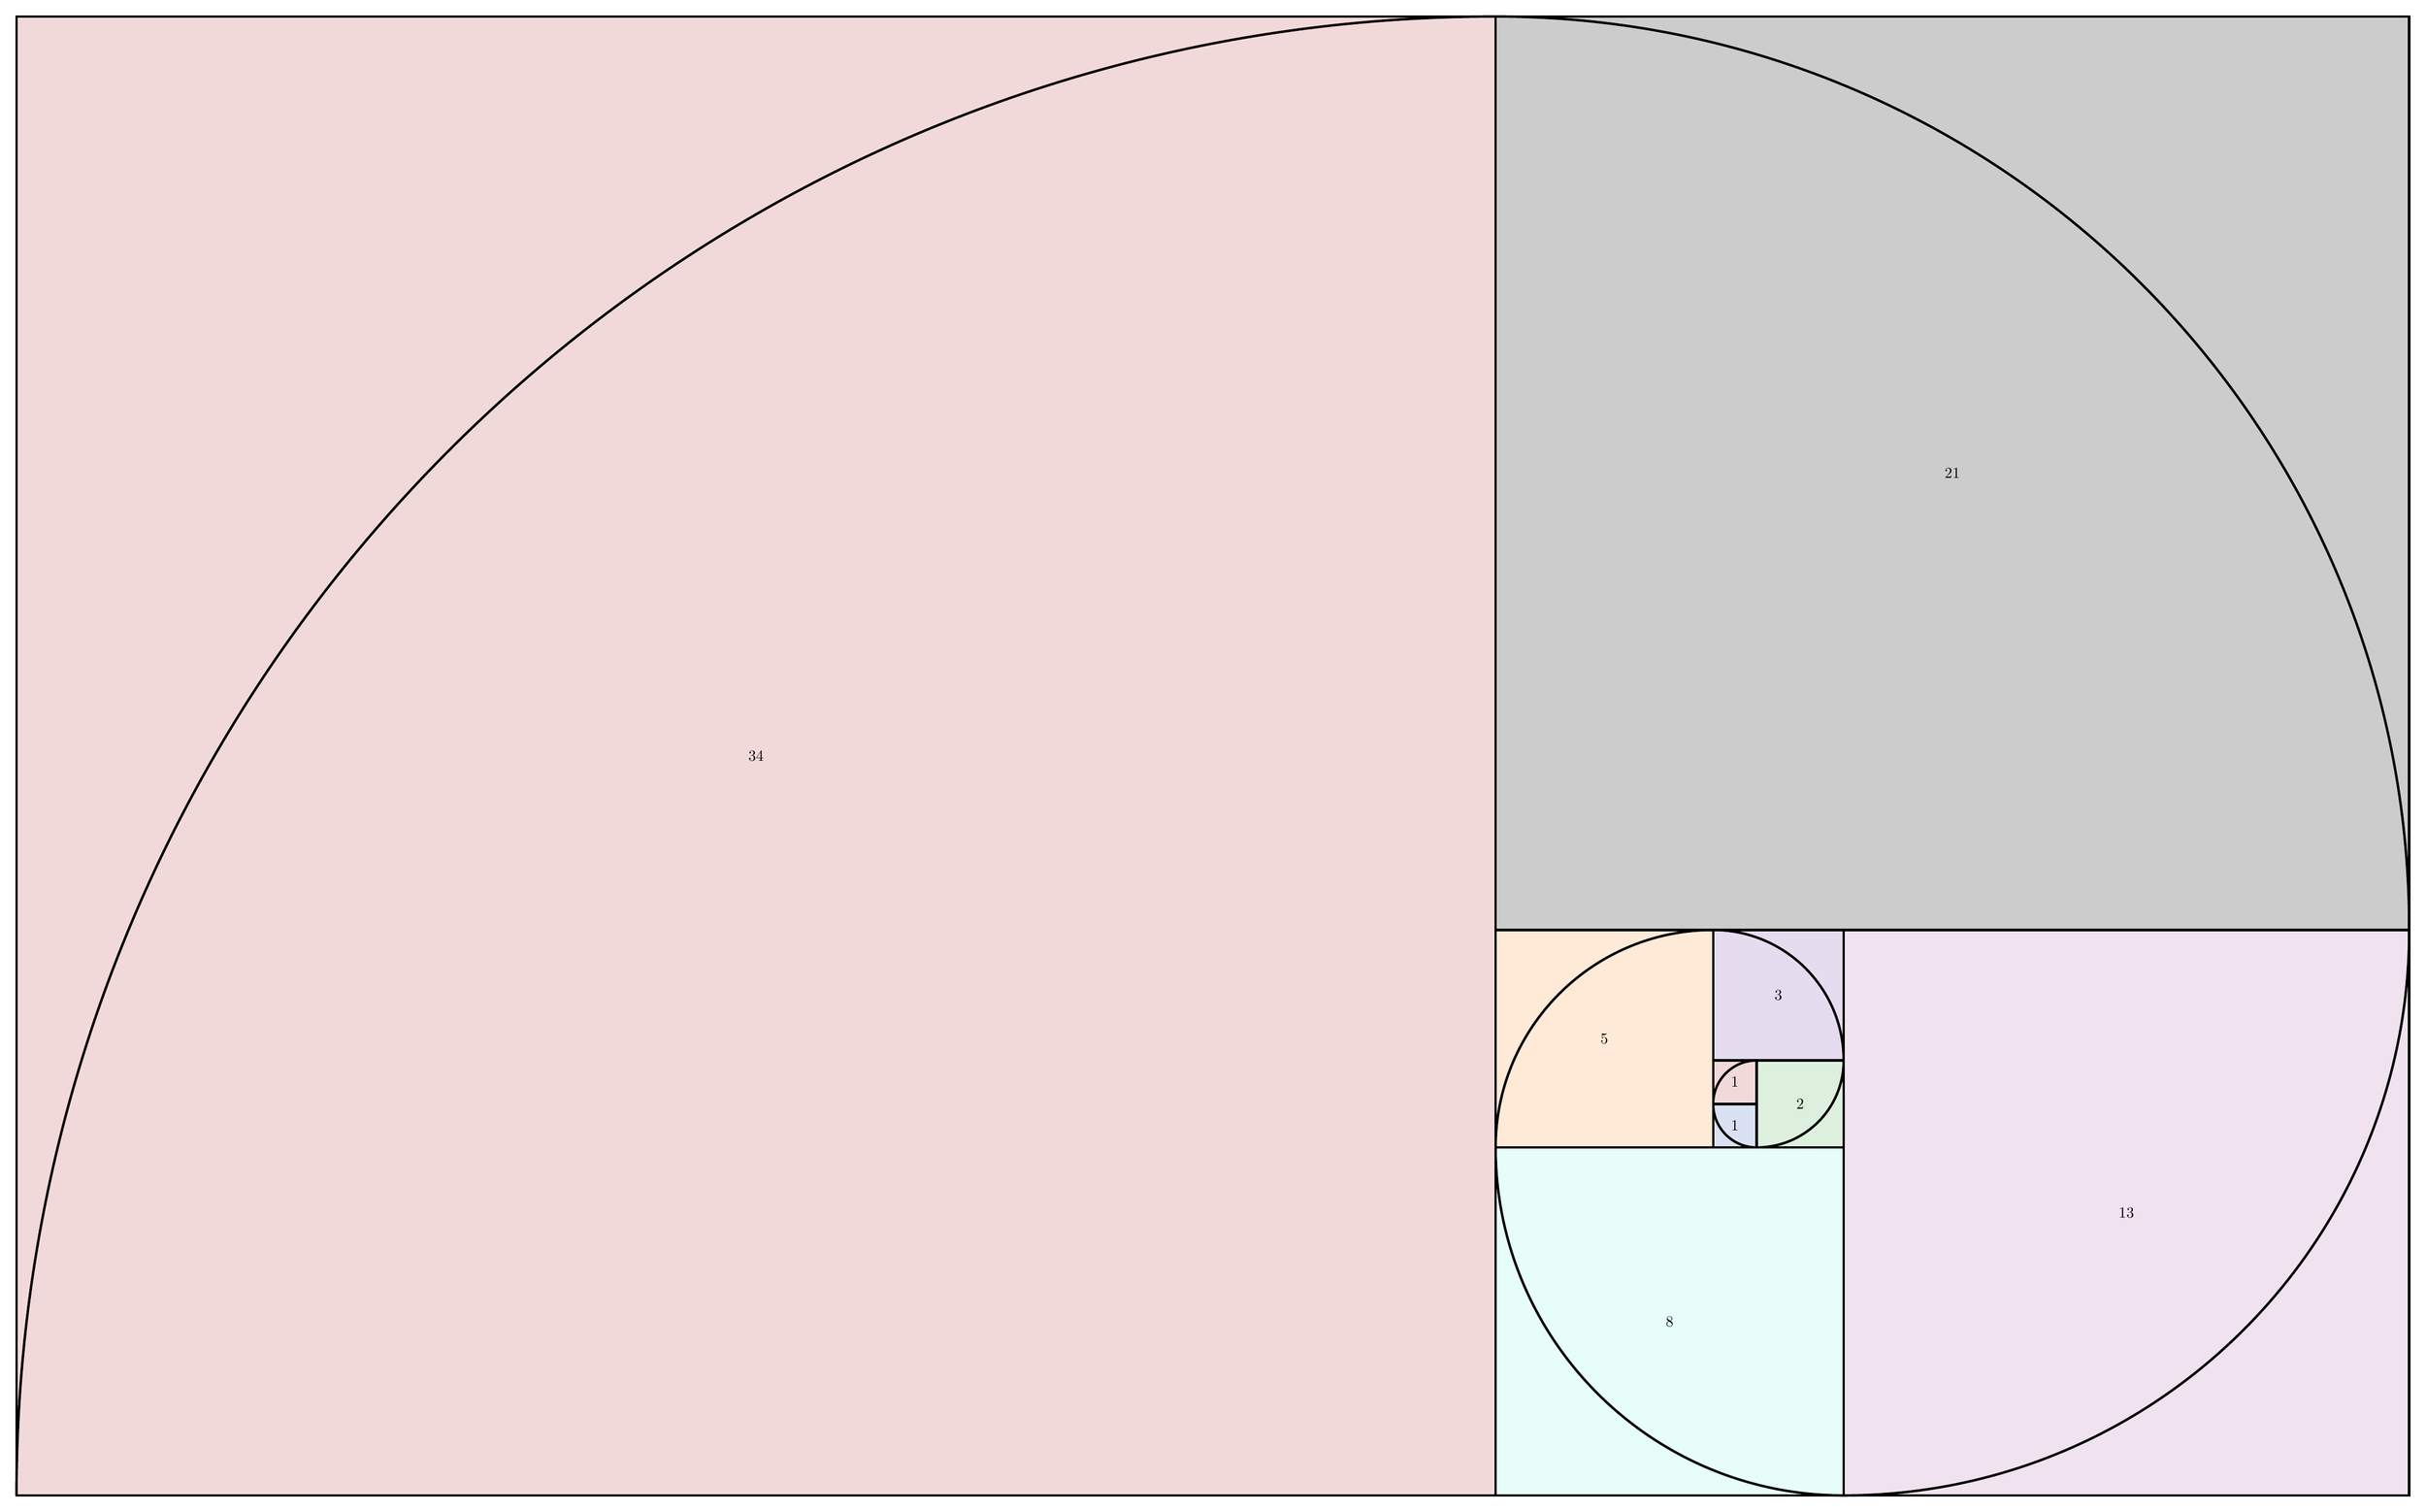
\begin{tikzpicture}[]
		\def\horizontal{{-1,-1,1,1}}
		\def\vertical{{1,-1,-1,1}}
		\def\center{{1,0}}
		\pgfmathsetmacro{\phi}{1.618033988749} % Golden ratio
		\pgfmathsetmacro{\x}{0}
		\pgfmathsetmacro{\y}{0}
		\foreach \n in {1,...,9}{
			% Calcs
			\pgfmathsetmacro{\k}{\n+1}
			\pgfmathsetmacro{\Fib}{int(ceil((\phi^(\k-1)-(\phi)^(-(\k-1)))/sqrt(5)))} % Fibonacci sequence
			\pgfmathsetmacro{\dx}{\Fib*\horizontal[mod(\n,4)]}
			\pgfmathsetmacro{\dy}{\Fib*\vertical[mod(\n,4)]}
			\pgfmathsetmacro{\dcx}{\center[mod(\n,2)]}
			\pgfmathsetmacro{\dcy}{\center[mod(\n+1,2)]}

			\coordinate (s) at (\x,\y);
			\coordinate (e) at ({\x+\dx},{\y+\dy});
			\coordinate (o) at ({\x+\dcx*\dx},{\y+\dcy*\dy}); % dx, dy, dx, dy, dx, dy, ...

			% Draw
			\pgfmathsetmacro{\m}{int(mod(\n,8))}
			\draw[ultra thick, fill=xcol\m!20] (s) rectangle (e) node[midway] {$\Fib$};
			\pic[draw, ultra thick, angle radius=\Fib cm] {angle=s--o--e};

			% Re-calc
			\pgfmathparse{\x+\dx}
			\xdef\x{\pgfmathresult}
			\pgfmathparse{\y+\dy}
			\xdef\y{\pgfmathresult}
		}
	\end{tikzpicture}
\end{document}
